
% THIS IS AN EXAMPLE DOCUMENT FOR VLDB 2012
% based on ACM SIGPROC-SP.TEX VERSION 2.7
% Modified by  Gerald Weber <gerald@cs.auckland.ac.nz>
% Removed the requirement to include *bbl file in here. (AhmetSacan, Sep2012)
% Fixed the equation on page 3 to prevent line overflow. (AhmetSacan, Sep2012)

\documentclass{vldb}
\usepackage{graphicx}
\usepackage{balance}  % for  \balance command ON LAST PAGE  (only there!)

% ****************** sungsoo's packages ****************************************
\usepackage{times}
%                              My Commands
\newcommand{\bi}{\begin{itemize}}
\newcommand{\ei}{\end{itemize}}
\newcommand{\be}{\begin{enumerate}}
\newcommand{\ee}{\end{enumerate}}
\newcommand{\ii}{\item}
\newtheorem{Def}{Definition}
\newtheorem{Lem}{Lemma}
\usepackage{algorithm}
\usepackage{algorithmicx}
\usepackage{algpseudocode}

\usepackage[]{algorithm2e}

\usepackage{graphicx}
\graphicspath{%
        {converted_graphics/}
        {./images/}
}
\usepackage{hyperref}
\usepackage{listings}
\usepackage{longtable}

% ****************** the following is needed for syntax highlighting
\usepackage{color}

\definecolor{dkgreen}{rgb}{0,0.6,0}
\definecolor{gray}{rgb}{0.5,0.5,0.5}
\definecolor{mauve}{rgb}{0.58,0,0.82}

\lstset{ %
  language=Java,                  % the language of the code
  basicstyle=\scriptsize,       % the size of the fonts that are used for the code
  numbers=left,                   % where to put the line-numbers
  numberstyle=\tiny\color{gray},  % the style that is used for the line-numbers
  stepnumber=1,                   % the step between two line-numbers. If it's 1, each line 
                                  % will be numbered
  numbersep=3.8pt,                  % how far the line-numbers are from the code
  backgroundcolor=\color{white},  % choose the background color. You must add \usepackage{color}
  showspaces=false,               % show spaces adding particular underscores
  showstringspaces=false,         % underline spaces within strings
  showtabs=false,                 % show tabs within strings adding particular underscores
  frame=false,                   % adds a frame around the code
  rulecolor=\color{black},        % if not set, the frame-color may be changed on line-breaks within not-black text (e.g. commens (green here))
  tabsize=2,                      % sets default tabsize to 2 spaces
  captionpos=b,                   % sets the caption-position to bottom
  breaklines=true,                % sets automatic line breaking
  breakatwhitespace=false,        % sets if automatic breaks should only happen at whitespace
  title=\lstname,                 % show the filename of files included with \lstinputlisting;
                                  % also try caption instead of title
  keywordstyle=\color{blue},          % keyword style
  commentstyle=\color{dkgreen},       % comment style
  stringstyle=\color{mauve},         % string literal style
  escapeinside={\%*}{*)},            % if you want to add a comment within your code
  morekeywords={*,...}               % if you want to add more keywords to the set
}
% ****************** end of sungsoo's packages ****************************************


\begin{document}

% ****************** TITLE ****************************************

%\title{A Sample {\ttlit Proceedings of the VLDB Endowment} Paper in LaTeX
%Format\titlenote{for use with vldb.cls}}

\title{Typical IT R\&R for the Data Warehouse}

% possible, but not really needed or used for PVLDB:
%\subtitle{[Extended Abstract]
%\titlenote{A full version of this paper is available as\textit{Author's Guide to Preparing ACM SIG Proceedings Using \LaTeX$2_\epsilon$\ and BibTeX} at \texttt{www.acm.org/eaddress.htm}}}

% ****************** AUTHORS **************************************

% You need the command \numberofauthors to handle the 'placement
% and alignment' of the authors beneath the title.
%
% For aesthetic reasons, we recommend 'three authors at a time'
% i.e. three 'name/affiliation blocks' be placed beneath the title.
%
% NOTE: You are NOT restricted in how many 'rows' of
% "name/affiliations" may appear. We just ask that you restrict
% the number of 'columns' to three.
%
% Because of the available 'opening page real-estate'
% we ask you to refrain from putting more than six authors
% (two rows with three columns) beneath the article title.
% More than six makes the first-page appear very cluttered indeed.
%
% Use the \alignauthor commands to handle the names
% and affiliations for an 'aesthetic maximum' of six authors.
% Add names, affiliations, addresses for
% the seventh etc. author(s) as the argument for the
% \additionalauthors command.
% These 'additional authors' will be output/set for you
% without further effort on your part as the last section in
% the body of your article BEFORE References or any Appendices.

\numberofauthors{1} %  in this sample file, there are a *total*
% of EIGHT authors. SIX appear on the 'first-page' (for formatting
% reasons) and the remaining two appear in the \additionalauthors section.

\author{
% You can go ahead and credit any number of authors here,
% e.g. one 'row of three' or two rows (consisting of one row of three
% and a second row of one, two or three).
%
% The command \alignauthor (no curly braces needed) should
% precede each author name, affiliation/snail-mail address and
% e-mail address. Additionally, tag each line of
% affiliation/address with \affaddr, and tag the
% e-mail address with \email.
%
% 1st. author
\alignauthor
Sung-Soo Kim\\ %\titlenote{Dr.~Trovato insisted his name be first.}\\
       \affaddr{Data Management Research Section}\\
       \affaddr{Electronics and Telecommunications Research Institute}\\
       \affaddr{128 Gajeong-ro, Yuseong-gu}\\
       \affaddr{Daejeon, South Korea}\\
       \email{\normalsize \it sungsoo@etri.re.kr}
% 2nd. author
%\alignauthor
%G.K.M. Tobin\titlenote{The secretary disavows
%any knowledge of this author's actions.}\\
%       \affaddr{Institute for Clarity in Documentation}\\
%       \affaddr{P.O. Box 1212}\\
%       \affaddr{Dublin, Ohio 43017-6221}\\
%       \email{webmaster@marysville-ohio.com}
% 3rd. author
%\alignauthor Lars Th{\Large{\sf{\o}}}rv{$\ddot{\mbox{a}}$}ld\titlenote{This author is the
%one who did all the really hard work.}\\
%       \affaddr{The Th{\large{\sf{\o}}}rv{$\ddot{\mbox{a}}$}ld Group}\\
%       \affaddr{1 Th{\large{\sf{\o}}}rv{$\ddot{\mbox{a}}$}ld Circle}\\
%       \affaddr{Hekla, Iceland}\\
%       \email{larst@affiliation.org}
%\and  % use '\and' if you need 'another row' of author names
% 4th. author
%\alignauthor Lawrence P. Leipuner\\
%       \affaddr{Brookhaven Laboratories}\\
%       \affaddr{Brookhaven National Lab}\\
%       \affaddr{P.O. Box 5000}\\
%       \email{lleipuner@researchlabs.org}
% 5th. author
%\alignauthor Sean Fogarty\\
%       \affaddr{NASA Ames Research Center}\\
%       \affaddr{Moffett Field}\\
%       \affaddr{California 94035}\\
%       \email{fogartys@amesres.org}
% 6th. author
%\alignauthor Charles Palmer\\
%       \affaddr{Palmer Research Laboratories}\\
%       \affaddr{8600 Datapoint Drive}\\
%       \affaddr{San Antonio, Texas 78229}\\
%       \email{cpalmer@prl.com}
}
% There's nothing stopping you putting the seventh, eighth, etc.
% author on the opening page (as the 'third row') but we ask,
% for aesthetic reasons that you place these 'additional authors'
% in the \additional authors block, viz.
%\additionalauthors{Additional authors: John Smith (The Th{\o}rv\"{a}ld Group, {\texttt{jsmith@affiliation.org}}), Julius P.~Kumquat
%(The \raggedright{Kumquat} Consortium, {\small \texttt{jpkumquat@consortium.net}}), and Ahmet Sacan (Drexel University, {\small \texttt{ahmetdevel@gmail.com}})}
%\date{30 July 1999}
% Just remember to make sure that the TOTAL number of authors
% is the number that will appear on the first page PLUS the
% number that will appear in the \additionalauthors section.


\maketitle

\begin{abstract}
Data warehousing is not new. Most large organizations have been investing
in data warehousing for years. Currently, cost-effective technology is creating
more possibilities for small and medium-size companies to build and deploy
data warehouse solutions too.

 There are many different roles on a data warehouse project that are filled by systems professionals. Many roles are consistent regardless of what kind of system is being developed. In this technical report, we describe the IT roles and responsibilities (R\&R) for a data warehouse project.
\end{abstract}

\section{Introduction}
 There are many stories about wild successes, and
just as many about failed projects. With so much buzz about datawarehousing,
it is often assumed that everyone already knows the basics. However, many people are being exposed to these concepts for the first time. To ensure a
common understanding, it is worth taking the time to boil things down to the
essence of data warehousing.

A \textit{data warehouse} (DW) is the collection of processes and data whose overarching
purpose is to support the business with its analysis and decision-making. In
other words, it is not one thing per se, but a collection of many different
parts. Before looking more closely at the specific parts of a data warehouse
environment, it is helpful to compare the characteristics and purpose of a data
warehouse with an operational application system.

Differences Between Operational and DW Systems
Applications that run the business are called \textit{online transaction processing systems}
(OLTPs). OLTP systems are geared toward functions such as processing
incoming orders, getting products shipped out, and transferring funds as
requested. These applications must ensure that transactions are handled
accurately and efficiently. No one wants to wait minutes to get cash from
an automated teller machine, or to enter sales orders into a company’s system.
In contrast, the purpose and characteristics of a data warehousing environment
are to provide data in a format easily understood by the business
community in order to support decision-making processes. The data warehouse
supports looking at the business data over time to identify significant
trends in buying behavior, customer retention, or changes in employee productivity.

Figure  \ref{fig:datawarehouse} shows the correct order to successfully design and implement a data warehousing environment. Both
the technical and business team members play a role throughout.

\begin{figure}[htb]
\centering
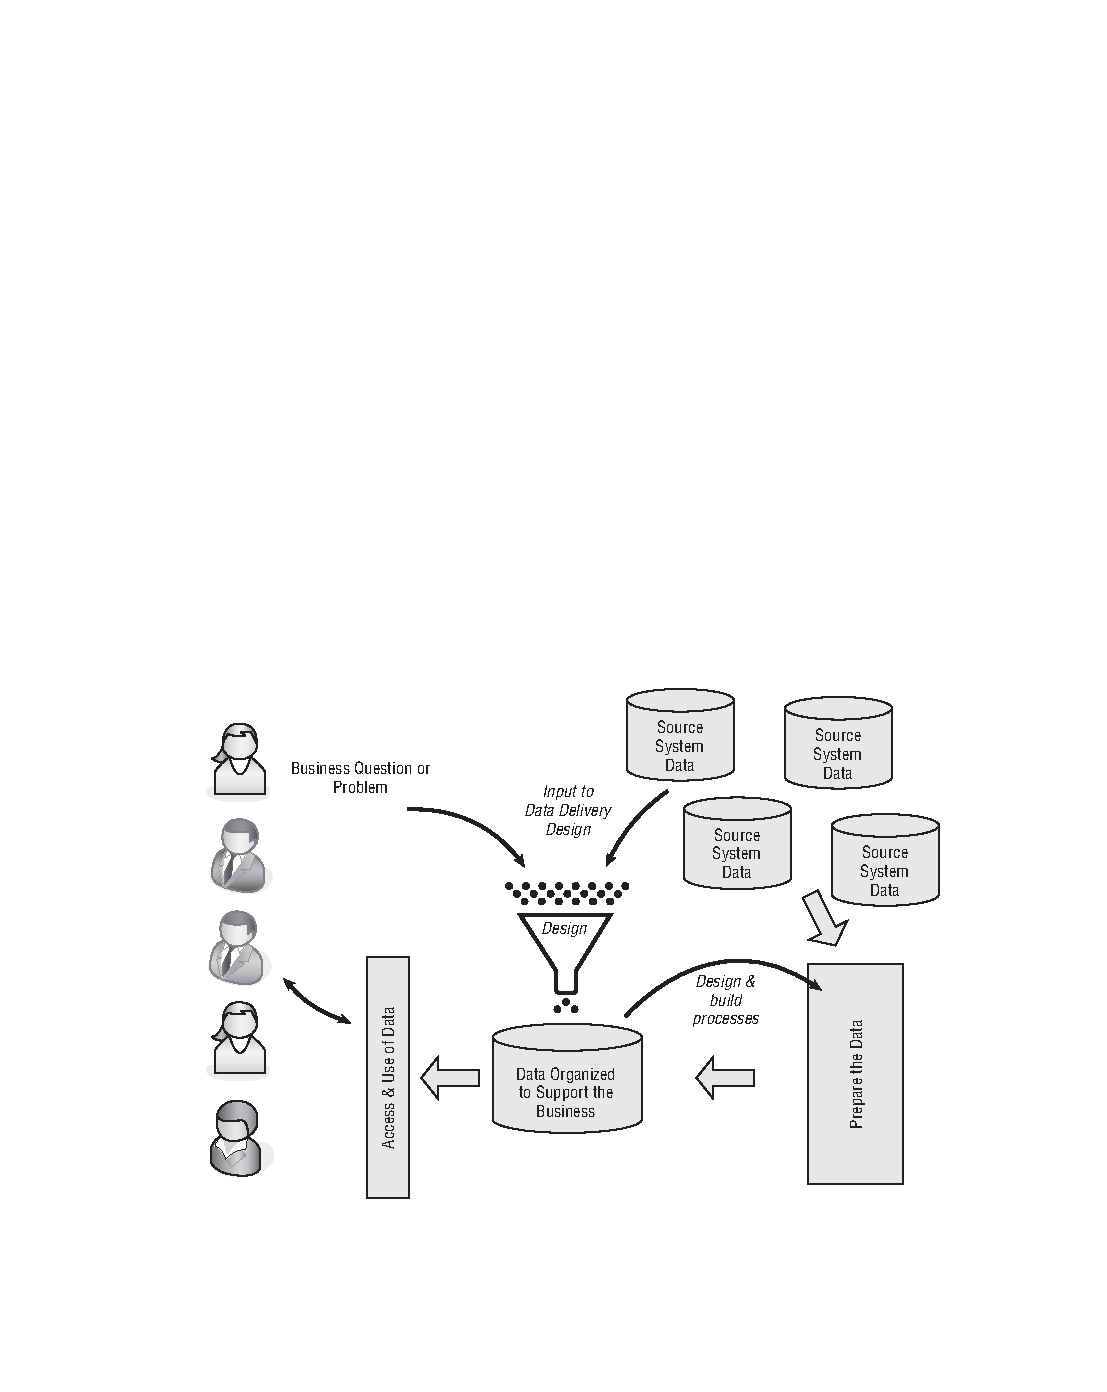
\includegraphics[width=0.48\textwidth]{datawarehouse}
\caption{Optimal data warehouse design and development sequence}
\label{fig:datawarehouse}
\end{figure}

The input of the business community is invaluable to a project team. Likewise, a data warehouse cannot be built without the talent, technical expertise, and rigor that the systems staff offers. The data warehousing industry has developed technologies and methods to design and implement robust environments that support businesses today and into the future. You must trust the technical team members to construct components to fit together to provide you with an environment that will support your business requirements. Let the systems staff do what they do best: make technical design decisions and build the capabilities. You really should not care which hash algorithm is used to load large tables into a database as long as you can get the data you need in a timely manner.

\section{CIO/IT Executive Sponsor}
The data warehouse should have one executive sponsor from the IT organization that will partner closely with the executive business sponsor. This is typically the CIO, but in large organizations this could be a senior manager in the IT organization. This person should be ultimately responsible for the technology side of the data warehouse and should have management responsibility over the IT staff on the data warehouse. This person usually shares the funding responsibility with the executive business sponsor and will own control for the technical aspects of the data warehouse environment. It is very important that the executive sponsors from the two organizations are seen as equals and that they are on the same page in terms of goals and objectives for the data warehouse. \cite{Reeves:DW}

\section{Data Warehouse Manager}
The data warehouse manager’s role represents the driving force behind the data warehouse environment from the IT organization. This individual is often given direct responsibility for the funds for the data warehouse project. This is the primary visionary for data warehousing in the organization, and the lead systems professional who is responsible for building and sustaining the data warehouse. The data warehouse manager continues to have responsibility for the data warehouse after a project is complete and oversees support, maintenance, and growth.

The data warehouse manager must set the overall direction of the data warehouse. This is done in conjunction with key business management. This includes making sure that a sound technical and data architecture is developed. The data warehouse manager is the focal point for blending industry best practices with internal best practices to develop an overall methodology and techniques that will ensure the long-term success of data warehousing within the organization. This includes adapting \textit{system development life cycle} (SDLC) practices and the definition of standard deliverables to meet the unique data warehousing needs.

If there are many data warehousing projects underway, the data warehouse manager would then be involved in coordinating and leveraging resources across the projects. These resources could include \textit{people} as well as \textit{technology} .

\subsubsection*{DESIRED CHARACTERISTICS OF THE DATA WAREHOUSE MANAGER}

\bi
\ii Sound analytical and reasoning skills
\ii Strong presentation and communication skills 
\ii Able to educate others
\bi
\ii IT: About the business and uses of the data
\ii Business: About datawarehousing, how the data looks, and what applications/reports are needed
\ei
\ii Understands the business
\ii Possesses project management experience
\ii Has exposure to the technologies involved
\ii Understands the organization’s culture and how things get done
\ii Exhibits leadership
\ii Understands and can manage risk
\ii Able to manage and coordinate multiple projects and priorities
\ei

\section{Business Systems Analyst}
The business systems analyst role is similar to the business analyst, but this person needs to have sound knowledge of data warehousing design principles. The business systems analyst will participate in, or even drive, the business requirements gathering process and will be a key player in building the partnership with the business community. The business systems analyst will also be expected to do the following:
Participate in the development of the dimensional model Help research data-related issues
Be a liaison between systems and the business communities for daily project tasks
Develop and oversee testing plans
Develop project documentation and deliverables
The business systems analyst role is often blended with the business analyst role. This is effective only if a single person can understand the business clearly enough and delve deeply enough into the details of data warehouse design and development.

\subsubsection*{DESIRED CHARACTERISTICS OF THE BUSINESS SYSTEMS ANALYST}
\bi
\ii Excellent problem-solving skills
\ii Understanding of business processes and functions
\ii Strong technical background
\ii Able to facilitate and communicate technical issues to a variety of audiences
\ii Understands the system development life cycle
\ii Good writing skills
\ii Quick learner
\ii Persistence to work through complex issues and design challenges
\ii Enthusiastic, motivated, and curious about learning the business
\ei

\noindent
\textbf{NOTE} The most important characteristic to look for in candidates for the position of business systems analyst for a data warehouse project is curiosity. If a person is sincerely interested in what the business does and how things work, then this will feed their ability to gather requirements and then translate them into a solution.

\section{Source System Analyst}
The source system analyst is not a full-time member of the data warehouse project team but plays a critical role. The data warehouse team must have one source system analyst designated for each source system that will feed the data warehouse. This person needs to have experience and knowledge of the underlying systems that will be used to populate the data warehouse. The source system analyst will also be expected to do the following:

\bi
\ii Support the development of the dimensional model
\ii Provide file layouts, data models, and data element definitions that exist for the source systems
\ii Research data-related issues
\ii Serve as the subject matter expert for the source system
\ei
When there is limited documentation for source systems, the source system analyst is often the only person who knows what each data element actually means. The names and how the source systems use each field may be a mystery without the active participation of this highly valuable resource.

\subsubsection*{DESIRED CHARACTERISTICS OF THE SOURCE SYSTEM ANALYST}
\bi
\ii Strong problem-solving skills
\ii Persistence to work through complex issues and design challenges
\ii Patience to support detailed, field by field analysis
\ii Willing to put forth extra effort to help the data warehouse initiative
\ii Understands the critical nature of his or her knowledge
\ii Able to juggle multiple priorities, including communicating to management concerns about the scheduling of their own time
\ii Shows interest in learning about data warehousing
\ei

\section{Data Modeler/Data Architect}
The data architect’s responsibilities are to develop a \textit{big picture strategy} for how data will be handled, stored, and processed to support the requirements of a specific project and to accommodate the requirements across the enterprise. 
This is the heart of the data warehouse. The data architect sets this vision. This includes driving or participating in the following:

\bi
\ii Defining the data structures and philosophy for the staging area 
\ii Defining the data structures and philosophy for the data warehouse 
\ii Participating in the requirements gathering process
\ii Understanding specific project requirements
\ii Gathering or researching enterprise data requirements and standards
\ii Ensuring that the data warehouse architecture fits in the overall enterprise data vision
\ei

Data modeling takes things to a lower level of detail. This entails understanding individual data elements and how they relate to each other; and then applying what was learned during the requirements gathering process in order to develop data models to support the business. There may be a need for detailed data modeling to support the staging and preparation processes. There is also a need for a dimensional model to reflect the specific data needed to support the business objectives of the project. The model must also be flexible enough to be extended as new data and requirements are discovered over time. The basics of a well-designed dimensional model should be able to sustain a data warehouse for years. The data modeler will be responsible for the following:

\bi
\ii Designing data models and databases to meet current and future needs
Understanding how the data model will support the business reporting and analyses
Researching data content and availability to ensure that the model is grounded in reality
Researching and recommending approaches to handle data integration
Performing detailed data analysis to understand the data as it currently exists
Developing logical database designs
\ei

\noindent
\textbf{NOTE} Dimensional modeling for a traditional data modeler can prove to be very challenging. If a data modeler or architect is fighting standard data warehousing practices, take action. Education may not be enough to change their ways. If this continues, consider reassigning that individual to a traditional project and get someone who will effectively support the data warehouse. That way, you can still leverage their skills and experience without causing delays and poor design choices for the data warehouse.

\subsubsection*{DESIRED CHARACTERISTICS OF THE DATA MODELER/DATA ARCHITECT}
\bi
\ii Understands the business requirements and the business point of view
\ii Understands the impact of data design on the rest of the project
\ii Understands data warehouse design best practices and approaches
\ii Understands how BI tools work and present information to users
\ii Understands the benefits and purpose of dimensional modeling and is an expert modeler
\ii Curious and motivated
\ii Able to communicate effectively with both business and technical groups
\ei

\section{ETL Developer(s)}
One of the most complex, challenging, and time-consuming parts of a data warehouse project is preparing the data for access and analysis. The main steps are to extract, transform, and load (ETL) the data. There are usually multiple systems professionals who perform the design and development of the ETL processes to populate the data warehouse. The lead ETL developer may sit in on requirements gathering sessions. It is also beneficial for the lead ETL developer to participate in the creation of the dimensional data model. This helps to ensure a full understanding of the complete model.

ETL developers work with the rest of the project team to define rules about how to clean, validate, and integrate the data. This often involves working directly with the business community. In some organizations, this must be done by working through the business system analyst. The ETL developers spend a lot of time researching and resolving issues discovered in the data as it is prepared for the data warehousing environment.


\subsubsection*{DESIRED CHARACTERISTICS OF THE ETL DEVELOPER}

\bi
\ii Ability to adapt when changes occur
\ii Understand the full data warehouse life cycle
\ii Appreciation and desire to work through data quality issues 
\ii Experienced system developer
\ii Ability and interest to learn new techniques and approaches 
\ii Creative problem solver
\ei

\section{Business Intelligence Application Developer}
The business intelligence application developer is responsible for creating and maintaining queries, reports, and applications. This usually involves using business intelligence (BI) tools. These tools need to be configured or set up properly to access the data mart. Each BI tool has a semantic layer, or metadata, that it uses to traverse the data and manage defined metrics. Once the BI tool is configured, a wide range of activities need to be performed, including the following:
\bi
\ii Designing and developing a suite of report templates
\ii Designing and developing a deployment strategy for reports
\ii Designing and developing performance dashboards or scorecards
\ii Designing and developing BI report and application documentation and training materials
\ii Supporting business users to help them increase their knowledge and use of the BI tool
\ei

\noindent
\textbf{NOTE} There may be two different types of BI developers. The first has deep technical skills and is responsible for installing and configuring the BI technology. They also design and deploy complex reports and analyses. The second type of BI developer is less technical and may be filled from the business community. This second role is responsible for creating reports and delivering analyses to support the business community. This second type often directly supports requests from
senior management.

\subsubsection*{DESIRED CHARACTERISTICS OF THE BI APPLICATION DEVELOPER}

\bi
\ii Strong understanding of the business requirements
\ii Interested in helping the business leverage the data warehouse
\ii Flexible and able to adapt to ongoing changing requests for information 
\ii Works well with the business community
\ii Good communication skills
\ii Able to translate business requests into BI report specifications
\ii Strong analytic abilities
\ei

\section{Other Supporting Roles}
A number of other technical roles are required for successful completion of a data warehousing project. These include a variety of technical functions, including database administration, security, network administration, systems architecture, training, testing, and operations support. These people are involved in making sure that the foundation technologies are set up and working properly and that the project is deployed successfully.
The roles for the business and IT communities have been described here individually, but the real strength of a data warehouse emerges when these people all work together. Ideas for helping to build and maintain this relationship are covered next.

\bibliographystyle{abbrv}
\bibliography{sqlonhadoop}

\end{document}
